\subsection{Kepler’s Second Law Emerges — Without a Word About Kepler}

Having built a calculus of motion from nothing but energy and symbols, Lagrange was ready to turn his gaze skyward.

He didn’t reach for Newton’s forces. He didn’t reach for Kepler’s ellipses. He didn’t even reach for a telescope.

Instead, he reached for his pen.

If the motion of a planet could be expressed in terms of energy, then planetary motion, too, could be tamed by his variational method. No geometry. No conics. Just a Lagrangian and a set of coordinates — the right ones.

When Lagrange turned his symbolic machinery toward planetary motion, he didn’t draw ellipses or trace conic sections. He didn’t mention Kepler. He didn’t need to. Instead, he chose two coordinates — not \( r \) and \( \theta \), but abstract symbols \( q_1 \) and \( q_2 \). One represented the radial distance from the sun, the other the angle swept out in the orbital plane.


\begin{figure}[H]
\centering
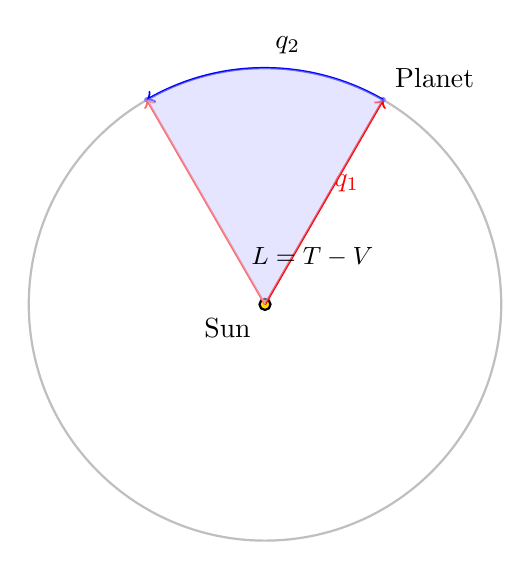
\begin{tikzpicture}[scale=3, 
    planet/.style={circle, fill=blue!50, inner sep=0pt, minimum size=2pt},
    sun/.style={circle, fill=yellow!80!orange, draw=black, thick, minimum size=4pt, inner sep=0pt}
]

% Draw the sun at the origin
\node[sun, label=below left:Sun] (sun) at (0,0) {};

% Draw orbital path (just a circular placeholder for abstraction)
\draw[thick, gray!50] (0,0) circle (1);

% Two sample positions of the planet
\coordinate (P1) at (60:1);
\coordinate (P2) at (120:1);
\node[planet, label=above right:Planet] at (P1) {};
\node[planet] at (P2) {};

% Radial vectors q1
\draw[->, thick, red] (0,0) -- (P1) node[midway, above right] {$q_1$};
\draw[->, thick, red!60] (0,0) -- (P2);

% Arc between positions (for q2)
\draw[thick, ->, blue] (P1) arc[start angle=60, end angle=120, radius=1cm];
\node at (85:1.1) {$q_2$};

% Equal area sector (hinting at Kepler's 2nd Law)
\fill[blue!20, opacity=0.5] (0,0) -- (60:1) arc[start angle=60, end angle=120, radius=1cm] -- cycle;

% Optional labels
\node at (0.2,0.2) {\small $L = T - V$};

\end{tikzpicture}
\caption{Lagrange’s abstract coordinates \( q_1 \) (radial) and \( q_2 \) (angular) applied to planetary motion. The shaded area represents equal area swept — a geometric consequence of conserved angular momentum.}
\end{figure}


Then he did what he always did: express motion as energy.

The kinetic energy, written in Lagrangian form, looked like this:

\[
T = \frac{1}{2} m \left( \left( \frac{dq_1}{dt} \right)^2 + a(q_1)^2 \left( \frac{dq_2}{dt} \right)^2 \right)
\]

Here’s what this expression is really saying — not just mathematically, but physically.

\begin{itemize}
    \item \( q_1 \) is the radial distance from the center — in our case, the sun. It tells us how far the planet is from the center of attraction at any moment in time. If this number changes, it means the planet is moving inward or outward — toward or away from the sun.
    
    \item \( q_2 \) is the angular coordinate — it tells us where the planet is in its orbit, like the hand of a clock sweeping around. Its rate of change, \( \frac{dq_2}{dt} \), measures how quickly the planet is sweeping through space — its rotational speed.
    
    \item \( a(q_1) \) is a function that acts like a lever arm. It translates the radial distance into a kind of “rotational radius.” In the simple case of polar coordinates in flat space, this is just \( a(q_1) = q_1 \), and so the term \( a(q_1)^2 \left( \frac{dq_2}{dt} \right)^2 \) becomes the familiar expression for rotational kinetic energy: \( r^2 \omega^2 \).
\end{itemize}

This whole expression is the total kinetic energy of the system. And what’s elegant about it is that it splits motion into two independent pieces:

\begin{itemize}
    \item The first term, \( \left( \frac{dq_1}{dt} \right)^2 \), is the energy from moving closer or farther from the center — the straight-line, in-and-out motion.
    
    \item The second term, \( a(q_1)^2 \left( \frac{dq_2}{dt} \right)^2 \), is the energy from sweeping around — the curved, angular motion.
\end{itemize}

Together, they form a symbolic expression of motion that doesn’t require drawing the orbit or computing forces. Lagrange didn’t care what shape the orbit was. He didn’t even need to name it. What mattered was how fast each piece of the system was changing — radially and angularly — and how much energy those changes carried.

\begin{quote}
\textit{Where Newton measured pushes and pulls, Lagrange measured motion itself — how much was happening, and where.}
\end{quote}

This formulation gave him the freedom to apply the same symbolic machinery to any system, whether it was a swinging pendulum, a rolling wheel, or a planet orbiting a star. Once you wrote down the kinetic and potential energies in terms of the system's coordinates, the rest followed from a single principle — no diagrams needed.

But then Lagrange noticed something strange — or rather, something beautifully ordinary: if a coordinate like \( q_2 \) doesn't appear explicitly in the Lagrangian, something magical happens.

Mathematically, this means:
\[
\frac{dL}{dq_2} = 0 \quad \Rightarrow \quad \frac{d}{dt} \left( \frac{dL}{d\dot{q}_2} \right) = 0
\]

In plain terms: if the system doesn’t “care” where it is around the circle — if rotating it doesn’t change its energy — then the \textit{generalized momentum} associated with that rotation stays constant.

In this case, that conserved quantity turns out to be:
\[
a(q_1)^2 \cdot \frac{dq_2}{dt}
\]
which is exactly angular momentum.

But angular momentum isn’t just a number — it’s geometry in motion. It tells us that planets sweep out equal areas in equal times. It tells us that a planet moves faster when it's close to the sun and slower when it's far, in just the right way to keep the area sweep rate constant.

In other words:
\begin{quote}
\textit{Kepler’s Second Law wasn’t proven. It was absorbed — hidden inside the algebra of symmetry.}
\end{quote}

Lagrange didn’t need a telescope. He didn’t need ellipses. He just needed structure. And when he saw that a coordinate disappeared from the Lagrangian, he knew: something must be conserved.

\subsubsection{Conservation Laws from Lagrangian Symmetry}

Lagrange’s real contribution wasn’t in computing new quantities — it was in showing that conservation itself could be read from the structure of your equations. If something doesn’t appear, it doesn’t change. If the system has a symmetry, there’s a law to be found.\footnote{These ideas were later formalized by Emmy Noether in 1918, who proved that every continuous symmetry of a physical system's action corresponds to a conservation law. Noether’s theorem unified and deepened the connection Lagrange had glimpsed — but the seeds were already in his work.}

\vspace{0.5em}

\begin{center}
    \renewcommand{\arraystretch}{1.5}
    \begin{tabularx}{\textwidth}{|l|X|X|}
    \hline
    \textbf{Symmetry in \( L \)} & \textbf{What It Means} & \textbf{What’s Conserved} \\ \hline
    \( q_i \) not in \( L \) & Coordinate is irrelevant to energy & Momentum conjugate to \( q_i \) \\ \hline
    Time appears only through \( q_i(t), \dot{q}_i(t) \) & No explicit time-dependence & Energy of the system remains constant \\ \hline
    No angular coordinate in \( L \) & Rotational symmetry & Angular momentum $\Rightarrow$ Equal areas swept \\ \hline
    \end{tabularx}
\end{center}

\vspace{1em}

And this is the genius of Lagrange: he didn’t reason from pictures. He reasoned from form. The structure of the Lagrangian whispered truths about motion — truths that Newton had to chase with diagrams and force vectors.

Lagrange didn’t just derive Kepler’s Second Law. He made it inevitable.
